\documentclass[]{article}   

\usepackage{graphicx}
\usepackage{xcolor} 
\usepackage{subcaption}
\usepackage{wrapfig}
\usepackage[utf8]{inputenc}
\usepackage{amsmath}
\usepackage{float}
%\usepackage{todonotes} 
\usepackage{color}
\usepackage{epstopdf}
\usepackage{mdframed}
\usepackage[a4paper]{geometry}
\geometry{top=3cm,left=4cm, right=4cm}

\sloppy
\definecolor{lightgray}{gray}{0.5}
\setlength{\parindent}{0pt}

\renewcommand{\figurename}{Figura}
\newcommand{\CP}[1]{\textcolor{blue}{#1}}

%SetFonts

%Title Page
\title{Tecnologia de control. \\ Disseny d'un controlador per un motor elèctric.}
\author{Guillem Casado, Albert Llebaria}
\date{Gener 2019}							

\begin{document}
\maketitle


\section{Objectius}

L'objectiu del present document és mostrar i analitzar els resultats obtinguts de la implementació d'un sistema de control per un motor elèctric emprant com a controlador un Arduino Genuino Uno. Per aconseguir-ho, es duen a terme els següents punts: 

\begin{itemize}
	\item Trobar una relació entre revolucions per minut i volts, ja que l'arduino treballa en aquestes últimes unitats.
	\item Obtenir el comportament de la sortida en rpm enfront a una consigna d'entrada en les mateixes unitats. 
	\item Estimar el model a controlar, amb les dades obtingudes en el punt anterior.
	\item Dissenyar un observador.
	\item Implementar un refús de pertorbacions constants emprant l'observador prèviament dissenyat. 
\end{itemize}

\section{Obtenció de la relació entre la sortida revolucions per minut i la entrada en volts}

Donat que l'Arduino treballa en volts i la consigna es dóna en revolucions per minut, cal trobar una relació entre ambdues variables. Per dur-ho a terme, es dona al PWM valors des de 40 fins a 255. Per cada unitat d'entrada, es guarda el valor de la velocitat de sortida, mitjançant una interrupció que llegeix el valor d'aquesta per cada flanc de pujada de l'encoder. Un cop es disposa de cada velocitat de sortida per cada entrada en el PWM, s'interpolen aquests punts mitjançant una corba de quart grau. La funció que defineix aquesta és la que s'utilitzarà per passar cada entrada en rpm a un número de màxim 8 bits que s'introduirà en el PWM. \\

/////IMATGES I ALGUN COMENTARI MÉS

\section{Estimació del model de la planta a controlar}

Per aquest cas en particular, no es disposa del model de la planta a controlar, ja que falta determinar alguns paràmetres d'aquest. Donat que aquest és necessari per al posterior control amb observador, es decideix estimar-lo. Per assolir-ho, en primer lloc es guarden valors de sortida en rpm obtinguts a partir de l'Arduino per diferents valors d'entrada també en aquestes unitats. A continuació, es compara la sortida real amb una simulada a través de Matlab. Els paràmetres del model a simular són introduits per la funció fminsearch, que anirà provant diferents valors d'aquests per tal que la diferència entre la sortida real i la simulada sigui mínima. Una vegada s'arriba a una solució òptima, es guarden els valors dels paràmetres del model de manera que aquest ja es podrà emprar per a dur a terme el control amb observador. \\

/////IMATGES I ALGUN COMENTARI MÉS

\section{Control amb observador}

Disposant doncs del model estimat, es procedeix a implementar el controlador. Donat que el model té dos estats i el motor només un sensor (velocitat), farà falta un observador. En primer lloc, es simula el control mitjançant el simulink. Proporcionant una entrada graó com a entrada i amb les constants del controlador //////////////////////////////////////////////////////////////////////VALORS DE LES CONSTANTS //////////////////////////////////////////////////////////////////////, s'obtenen els resultats de mostrats en la figura //////////X. Tal com es pot veure, el fet de que els pols tinguin part complexa provoca una petita oscil·lació en la sortida però el sistema segueix l'entrada perfectament. Així doncs, es procedeix a implementar el control en el propi arduino. El resultat de l'execució es mostra en la figura //////////X. Observant aquests, es dedueix que la sortida sempre està a un valor constant de la consigna. ///////AIXÒ ÉS DEGUT A....////////. El fet que aquesta diferència sigui pràcticament constant en qualsevol instant de temps, permet que es pugui solucionar mitjançant un refús de pertorbacions constants amb l'observador ja implementat. \\ 

/////IMATGES I ALGUN COMENTARI MÉS


\section{Control amb observador amb refús de pertorbacions constants}

La última millora a dur a terme consisteix en corregir la diferència constant entre entrada i sortida mitjançant un observador amb refús de pertorbacions. Es comença simulant el nou controlador amb Matlab. La resposta del sistema és idèntica a l'obtinguda a la simulada sense refús de pertorbacions i que es mostra en la figura ////////X. Això es degut a que en el model simulat no apareixen aquestes pertorbacions. D'aquesta manera, per valorar que aquest està funcionant s'ha d'implementar en el sistema real, és a dir, en l'Arduino. Els resultats de l'execució del nou codi es mostren en la figura ////////X. S'aprecia que l'observador està funcionant bé ja que les pertorbacions constants han deixat d'existir. \\

Tot i així, continuen havent-hi algunes possibles millores. En primer lloc, en cada flanc de pujada apareix un pic molt exagerat. Aquest es degut a //////////PQ??//////////. Per solucionar-lo, es limiten els valors que pot prendre la sortida per tal que no es dispari cada vegada en aquest punt en concret. Això provocarà que hi hagi certs valors de velocitat que no es podran obtenir però es considera que mai s'utilitzaran i, per tant, es suavitza el flanc de pujada per els valors en que es decideix que el motor pot treballar. Una altra millora seria refusar les pertorbacions sinusoïdals que apareixen en la sortida mitjançant un observador que les refusi. Aquestes són degudes al frec entre el sistema de reduccions del motor i l'excentricitat del rotor intrínseca de qualsevol procés productiu. Aquesta, a diferència de la primera, no s'ha pogut implementar. Malgrat això, el disseny de control dut a terme aconsegueix que la sortida segueixi pràcticament la referència (a pesar de les pertorbacions sinusoïdals) i de manera ràpida, ja que reacciona força bé a cada flanc de canvi de l'entrada graó. \\ 

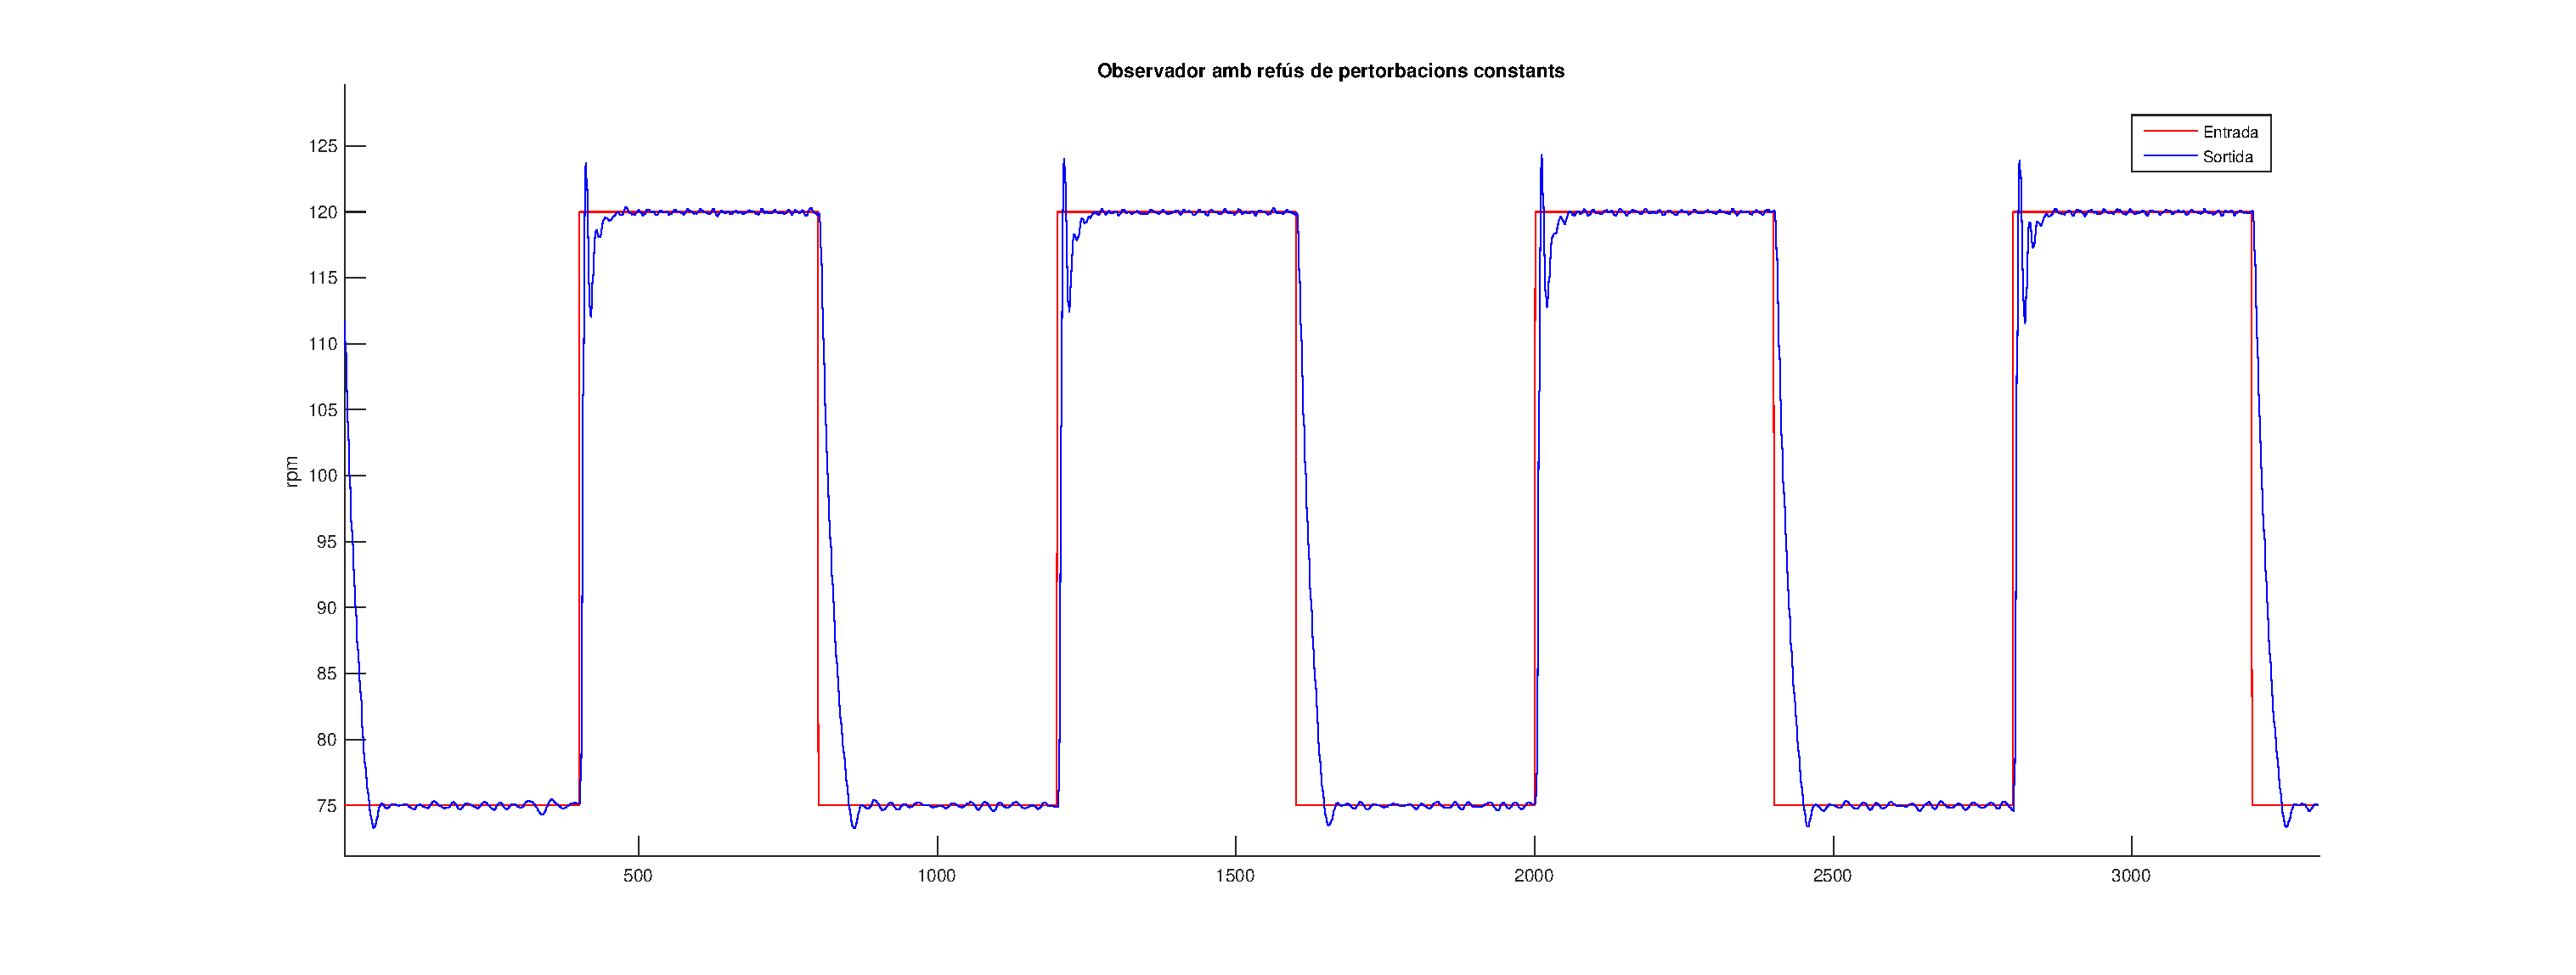
\includegraphics[scale=1]{Entrada_Sortida_Refus_Constant.eps} /////IMATGES I ALGUN COMENTARI MÉS


\end{document}